\documentclass[10pt]{report}
\usepackage[small,labelfont=it,textfont=it]{caption}
\usepackage{amsmath,
  alltt, amssymb, xspace, times, epsfig, algpseudocode, color,
  multirow, listings, graphicx, caption, subcaption, hyperref,
  appendix}
\usepackage[margin=2.5cm]{geometry}

\setlength{\evensidemargin}{0in} \setlength{\oddsidemargin}{0in}
\setlength{\textwidth}{6.5in} \setlength{\textheight}{8.5in}
\setlength{\topmargin}{0in} \setlength{\headheight}{0in}

\title{CS536 Final Project}
\author{Josh Reese, Nadya Ortiz}

\begin{document}
\maketitle

\section{Goals}
In this project our aim was to mimic distributed file transfers in
a simulated data center topology. From these transfers we look to
measure the time it takes for all receivers to complete using both TCP
and MPTCP (with varying degrees of subflows). Our interest here is
under what scenarios MPTCP is useful and when does it not provide any
benefit. In addition to this, when we find that MPTCP is useful how
much difference does it make in these scenarios? What we excpet to show
here is that in a data center environment where there is a large
amount of traffic and / or congestion we can see benefits to
allowing nodes to send across different paths using MPTCP. 

\section{Motivation}
in data centers there are often multiple paths between two nodes. If
the network gets congested under TCP this can cause the amount of time
a transfer will take to suffer greatly. This congestion can easily
occur in TCP if there are a large number of senders and receivers and
the senders have chosen routes that overlap, or are the
same. However, if a sender has multiple paths to each receiver it can
utilize those to help avoid congestion
in the network and reduce the amount of time to transfer the file. The
ideas behind MPTCP can be found in \cite{mptcp}. We used this work as
the initial building block for our idea. We then came across some work
done at Stanford which investigated various properties of a data
center topology under TCP and MPTCP \cite{datacenter} which provided
us with a working version of MPTCP for Mininet and a topology to begin
working with. 

\section{Original Results}
\label{sec:oresults}
In this experiment \cite{datacenter} the authors created an
implementation of MPTCP
inside of Mininet which they used to test and verify the results from
\cite{mptcp}. To do this they use an ECMP hashed routing protocol which
is implemented in the riplpox controller inside of Mininet. To run these
experiments, which include throughput, RTT, CPU utilization, and queue size,
they created a Fat Tree topology in which to peform each test. A diagram of
which can be found in Figure~\ref{fig:ft}. From this work we
took the Fat Tree topology and used this to run our tests as well. We
also use the MPTCP implementation from here. Code for this project and
the mptcp setup can be found at
\url{https://github.com/bocon13/mptcp_setup} and 
\url{http://github.com/bocon13/datacenter_mptcp}. This work helped
provide us with a framework for testing as well as a topology to use
in the final analysis.

\section{Our Goals}
The first goal of our project was to obtain the code from the two
projects discussed in Section~\ref{sec:oresults} and set up a working
version of their MPTCP implementation using Mininet 2.0.0. The initial
configuration required is an installation of their kernel update and a
verification to see if it is working correctly. This takes the form of
an N-switch 2-host topology, which we later used for the initial
phase of testing. Followed by
this the authors provide a working Fat Tree topology. It was our goal
to use both of these topologies for testing. From here we would try to
implement a third data center topology of our choosing and gather
results from that as well.

Once these topologies were set up and our tests able to run our main
goal was to investigate the impact TCP and MPTCP have on varying
workloads in these environments. To accomplish this we constructed
a very simple sender / receiver scenario which transfers a file (or
files) from one or more senders to one or more receivers. In this way
we were able to vary the amount of traffic introduced into the network.

\section{Results}
\subsection{Setup}
To conduct our experiments we set up a simple sender and receiver
scenario which could be scaled to multiple senders and multiple
receivers. Each sender will simply read in a file of size 50M and send
a portion of it to each receiver present. Meaning if this is a 1
sender 1 receiver workload the sender will receiver all 50M of
data. If we are using a 1 sender 2 receiver workload then each receiver
will receiver 25M of the original data. Each sender will send 500
lines of its file at a time (roughly 64KB of data) and the receivers
buffer has been set to 65536 to accommodate this. In addition to this
we use the N-switch 2-host topology from
\url{https://github.com/bocon13/mptcp_setup} and the Fat Tree topology
from \cite{datacenter} to run our workloads. All experiments were
conducted on Mininet 2.0.0 using the 3.5.0-89-mptcp patched kernel
from \url{https://github.com/bocon13/mptcp_setup}. The machine used to
conduct these experiments was a MacBook Air running OS X 9 with a 1.3
GHz core i5 processor and 4GB 1600MHz DDR3 memory. A detailed
explanation of the implementation as well as some specifics about how
the workloads were created can be found in
Section~\ref{sec:imp}. 

\subsection{N-switch 2-host}
\label{sub:res1}
For the first series of tests we examined the N-switch 2-host topology
with switches ranging from 2 to 5 and subflows ranging from 1 to the
number of switches present. In these tests we have 1 sender and 1
receiver connected to variable amounts of switches and we examine the
time it takes to transfer a file of size 50M between the two.

\begin{figure}[hb]
  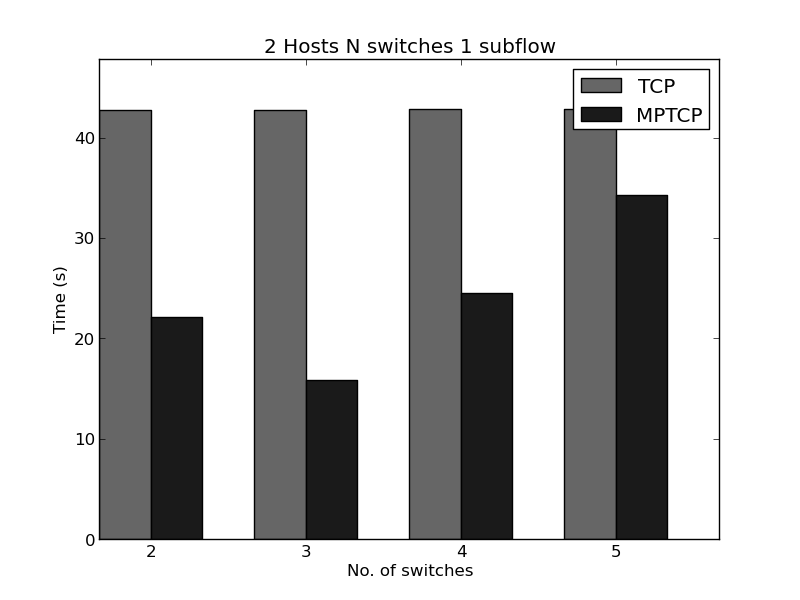
\includegraphics[width=\textwidth,height=4in]{images/hist_all.png}
  \caption{Time vs number of switches for 1 subflow.}
  \label{fig:swvt}
\end{figure}

\subsection{Fat Tree Topology (k=4)}
\label{sub:res2}
In the second series of testing we ran our sender / receiver
implementation on the Fat Tree topology (of k=4) with various number of senders
and receivers. One point to note is that we found cases where the
limitations in our system, either in hardware or with Mininet,
prevented us from running some tests. This occurs when there are too
many flows coupled with multiple senders and receivers. Specifically
we noticed this cases of more than 5 senders, 6 receivers, and 7 to 8
subflows. Similar issues were discovered in \cite{datacenter}
regarding CPU limitations on their system. In these cases we don't
report results for these tests because the results are unpredictable
and thus don't reliably represent the experiment. We represent these
results in individual charts by number of receivers (1 to 6) with time
to transfer a file (in seconds) on the y-axis and number of subflows
on the x-axis. Each line in the graph corresponds to a different
number of senders. In all of these graphs the point on the y-axis (1
subflow) represents the time to transfer the file(s) under TCP while
the remaining points represent the transfer time with MTPCP and the
corresponding number of subflows. These charts can be found in
Appendix~\ref{sec:app}. 

\section{Interpretation of Results}
In the tests presented in Section~\ref{sub:res1}, specifically
Figure~\ref{fig:flowvt}, we can examine the
graphs that test number of flows vs. time. From these graphs we can
see that adding 1 additional subflow can drastically decrease the
transfer time between the 2 hosts. However, when the number of flows
increases to above 1 the implementation appears to revert back to
TCP. This is something we couldn't figure out and spent some time
examining but never came to any conclusions. If we examine
Figure~\ref{fig:swvt} we can see a much clearer picture of the
benefits of using MPTCP in this topology. In this graph we show that
with more paths between the sender and receiver MPTCP can effectively
cut the transfer time in half. Another thing to note is that as the
switches increase past 3 the time to transfer using MPTCP tends to
increase. Our intuition regarding the cause of this suggests two
possible scenarios: the first is that on the senders side the number
of paths available is increasing and thus the sender will have to
monitor more paths according to the MPTCP protocol. On the other side
of the transfer, the receiver is likely receiving more information
simultaneously from all the switches and the threads performing the
receiving are forced to switch back and forth rapidly. 

If we now look at Figures~\ref{fig:rcv1}-\ref{fig:rcv6} we can see
some interesting results. In Figure~\ref{fig:rcv1} we see there is
really no advantage to using MPTCP regardless of the number of
senders. Our assumption here is that the traffic is congested in the
switch located directly above the host in this topology since all
senders are sending to only one location. In graphs past
Figure~\ref{fig:rcv2} we no longer use subflows above 6 due to the
limitation previously mentioned. Starting with this plot we can begin
to see some advantages to using MPTCP (specifically here for eight
senders). As the number of receivers increases we can more clearly see
the advantages to using MPTCP over TCP. In some cases decreasing the
transfer time by approximately 30\%. These results appear to support
our initial assumptions very nicely. We can see that as the number of
receivers increase, thus giving the senders more options regarding
possible paths, we are able to begin to see the benefits of using
MPTCP. Table~\ref{tab:times} provides a concise presentation of the
times taken for 3, 4, 5 and 6 receivers and the maximum amount of
senders our system could handle for those receivers. Here we report
specific times for TCP and MPTCP with 2, 3, 4 and 5 subflows. From
this table we can clearly see that in the 4 and 5 receiver tests
creating even 1 addition subflow can cause the transfer time to
drastically decrease (79s to 53s for 5 receivers).


\section{Challenges}
The first obstacle in this project was getting a working version of
Mininet with MPTCP up and running. From here we had to understand the
code used in \cite{datacenter} which included two fairly extensive
python files controlling the routing in the network and the design of
the topologies. Each of these files contained dependencies on various
Mininet components requiring us to dig deep into the internals of the
system to try to understand what was going on. When we had our initial
system running and were performing our early tests we noticed we
couldn't obtain any performance increase from using MPTCP. This caused
a bit of a
panic and we came to the conclusion that the edge switches inside the
Fat Tree were causing too much of a bottleneck for our file
transfers. From here we developed an entirely different topology, a
Dual Homed Tree, which we found in \cite{mptcp}\cite{dht}. We
struggled with the Dual Homed Tree, shown in Figure~\ref{fig:dht} for
some time, changing naming
conventions and interfaces and struggling with the riplpox controller
inside Mininet. We finally discovered from \cite{scalable} that
our routing might be wrong. This gave us key insights into
implementing a functioning version of the Dual Homed Tree. In the end
however, we were unable to obtain any results from this topology due
to limitations in connecting multiple interfaces from a host to
separate switches inside of Mininet. Even after we had this new
topology set up we spent a lot of time examining the output of the
controller to see if hosts were actually taking multiple paths in
their file transfers. One additional issue we encountered during the
development of the Dual Homed Tree was a situation where Mininet
entered a state in which it wasn't able to cleanup all the links and
switches it had created. We investigated through searching the
documentation and FAQs and posted onto the mailing list. In the end we
found out it was a kernel bug.

During the testing process we encountered a very large number of
errors. The most daunting of these was the amount of time required to
perform these tests. Due to the length of time for some of the
transfers we were unable to perform multiple executions of the test to
generate more accurate results. Once we started testing and really
stressing the system we noticed that on occasion Mininet would stop
responding and a transfer could continue indefinitely. This occurred
as the receivers increased and in flows of size seven and eight. At
this point we would need to reboot the system and begin the test at
the last stable checkpoint. This explains some of the unexpected
points of data in our plots. Some of these challenges are also
mentioned in \cite{datacenter} and are intrinsic to Mininet itself. In
addition to this we found that sometimes even for tests with low
stress on the system we would generate unexpected results. This could
be due to any number of factors, including issues with Mininet not
being properly cleaned up from previous tests.

\section{Implementation}
\label{sec:imp}
Code and instructions for recreating the tests from this project cane
be found at: \url{https://github.com/jreeseue/mptcp}. A dataset is
provided under the data/covtype directory to use for testing. There are
several files of note in this implementation.
\begin{itemize}
\item {\bf sender.py:} This file contains the code for a node to send
  its data. A sender takes an ID (used to read its file), a chunk size
  (unused), a dataset (unused but could be used to support different
  files in the future), and a list of IP addresses to send to. A
  sender will transfer its file, or a portion of its file, to each
  receiver in its list of IPs. Each sender will send 500 lines of data
  (approximately 64KB in this dataset) at a time until it has finished
  its transfer.
\item {\bf receiver.py:} This file contains the code for a node to
  receive data from one or more senders. A receiver takes an ID (used
  to save its data), a chunk size (unused), the number of receivers,
  the number of senders, and the name of the dataset as
  parameters. Each receiver will listen for connections and create a
  thread for each incoming connection. These threads will correspond
  to each sender in the test and will receive data until all the
  senders have completed their transfers. Each receiver has a buffer
  of size 65536 to correspond to the approximate 64KB each sender will
  be sending in each transmission. Once all senders are finished all
  receivers will write their received files to the disk.
\item {\bf test\_ft.py:} This file contains the code to test the
  implementation of the Fat Tree topology using the sender and
  receiver code previously described. Here we set up Mininet and
  attach it to the riplpox controller for routing, construct custom
  links, and create the mappings between senders and receivers. In an
  attempt to distribute the workload throughout the network we ensure
  that senders and receivers and never located in the same pod. To do
  this we assign pods 0 and 2 to senders and pods 1 and 3 to
  receivers. When a test is run senders and receivers are chosen at
  random from these pods.
\item {\bf dctopo.py:} This is a modified Fat Tree topology file from
  \url{https://github.com/bocon13/datacenter_mptcp}. The only changes
  to this are the Dual Homed Tree topology we've added at the end
  (which currently doesn't function). This is the topology used for
  testing the Fat Tree.
\item {\bf run\_test.py:} A script to run the workload of tests for
  the Fat Tree. Senders 1 to 8, receivers 1 to 8, and flows 2 to
  6. Not all of these tests were able to run on our system.
\item {\bf run\_switch.py:} A script to run the workload of tests for
  the N-switch 2-host setup. Switches ranging from 2 to 5.
\end{itemize}

\section{Conclusion}
From examining the work presented here we can see very clear benefits
to using MPTCP in a data center which has a high volume of traffic and
congestion. As we demonstrated with the increasing amount of receivers
we see also an increasing benefit to using MPTCP to transfer a
file. In addition to this we can see that for all the tests we
performed when the number of subflows reached four the time to
transfer stopped decreasing. This suggests either our system wasn't
able to properly handle flows above four or in this test set up four
subflows may be optimal in most cases. To conclude, the benefits to
using MPTCP in a higher volume data center may be very significant.

\section{Future Work}
There are several possible ways in which this work could be
expanded. This first, and most obvious of which, would be to implement
other data center topologies inside of Mininet and perform a
comparison between those and the Fat Tree used here. This could
provide us with an interesting comparison between how the physics
layout of a data center might have an impact on the effectiveness of
using MPTCP. While we tried to implement the Dual Homed Tree topology,
there wasn't enough time to get this running and perform the
tests. Two other topologies we examined were VL2 and the
B-Cube. Either of these two might prove to be an interesting
comparison to the Fat Tree, or each other. In addition there are
various parameters inside of Mininet that could be tweaked for
measurements. These include the bandwidht of links and size of packets
allowed in the queue of each switch (measured in
\cite{datacenter}). Once again these parameters might provide
interesting results when moving from TCP to MPTCP. As a modification
to the code we produced here an interesting change might be in the
amount of data a sender will send at a time and the size of a
receivers buffer. The values we set were initially fairly large (64KB)
and it might prove interesting to measure the impact different buffer
sizes (and send amounts) might have in these environments.

\begin{appendices}
  \chapter{Plots}
  \label{sec:app}

  \begin{figure}[hb]
    \centering
    \begin{subfigure}[b]{0.49\textwidth}
      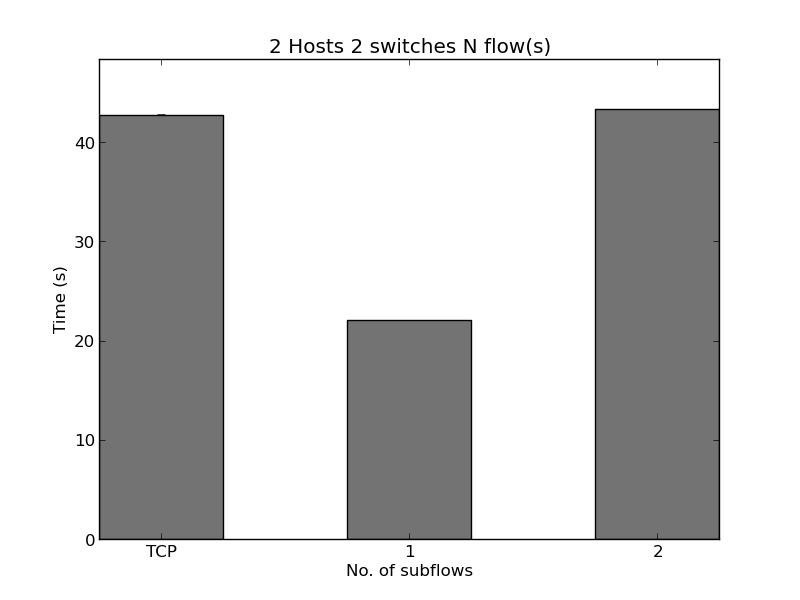
\includegraphics[width=\textwidth]{images/hist_sw2.png}
    \end{subfigure}
    \begin{subfigure}[b]{0.5\textwidth}
      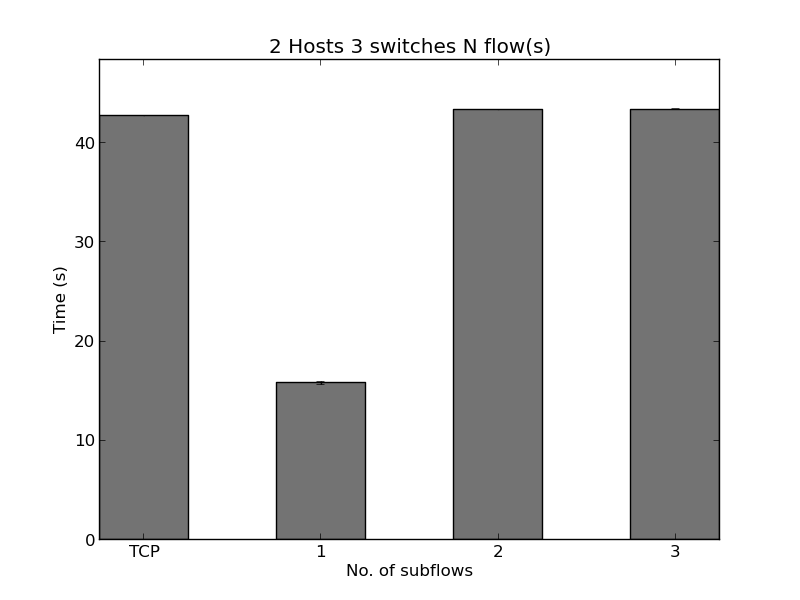
\includegraphics[width=\textwidth]{images/hist_sw3.png}
    \end{subfigure}
    \begin{subfigure}[b]{0.49\textwidth}
      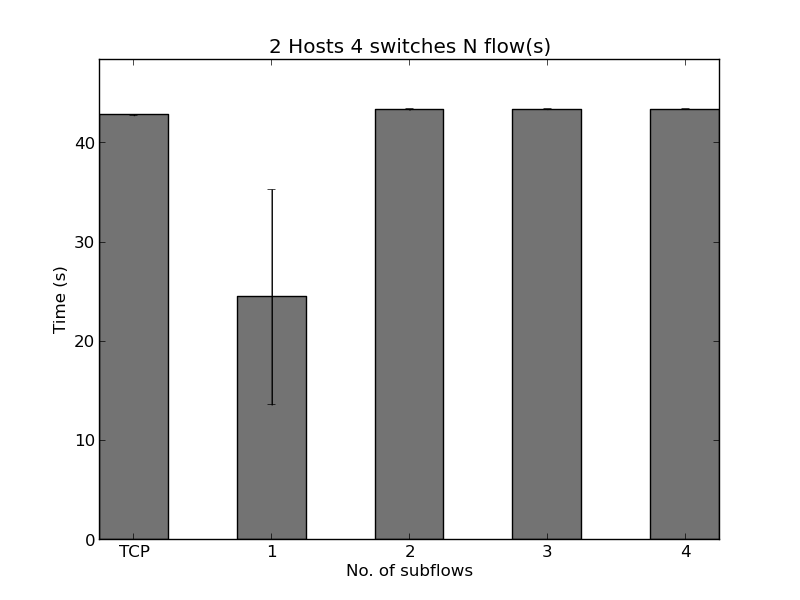
\includegraphics[width=\textwidth]{images/hist_sw4.png}
    \end{subfigure}
    \begin{subfigure}[b]{0.5\textwidth}
      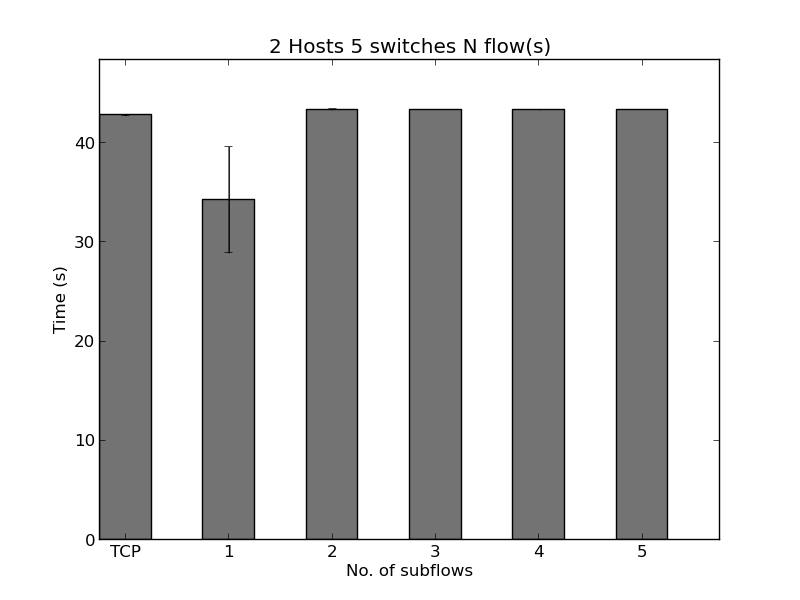
\includegraphics[width=\textwidth]{images/hist_sw5.png}
    \end{subfigure}
    \caption{Time vs. Number of flows for switches ranging from 2 to 5.}
    \label{fig:flowvt}
  \end{figure}

  \begin{table}
    \captionsetup{width=0.8\textwidth}
    \begin{center}
      \begin{tabular}{|c|c|cccccc|}
        \hline
        \# Recv & \# Sndr & TCP & 1 Flow & 2 Flows & 3 Flows & 4 Flows & 5
        Flows \\
        \hline
        3 & 5 & 87 & 77 & 80 & 79 & 77 & 81 \\
        \hline
        4 & 5 & 77 & 72 & 64 & 65 & 65 & 65 \\
        \hline
        5 & 5 & 79 & 53 & 50 & 50 & 52 & 56 \\
        \hline
        6 & 5 & 62 & 53 & 53 & 50 & 53 & 50 \\
        \hline
      \end{tabular}
      \caption{Number of receivers with the maximum number of senders
        that could be used during testing. Times reported are for TCP
        and the various number of subflows.}
      \label{tab:times}
    \end{center}
  \end{table}

  \begin{figure}[!b]
    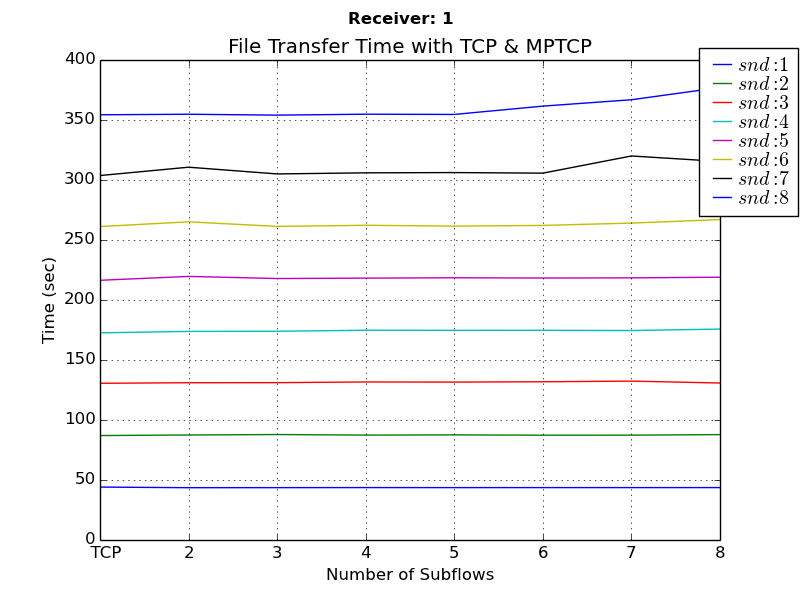
\includegraphics[width=\textwidth,height=3.8in]{images/rcv_1.png}
    \caption{1 receiver multiple senders.}
    \label{fig:rcv1}
  \end{figure}

  \begin{figure}[!b]
    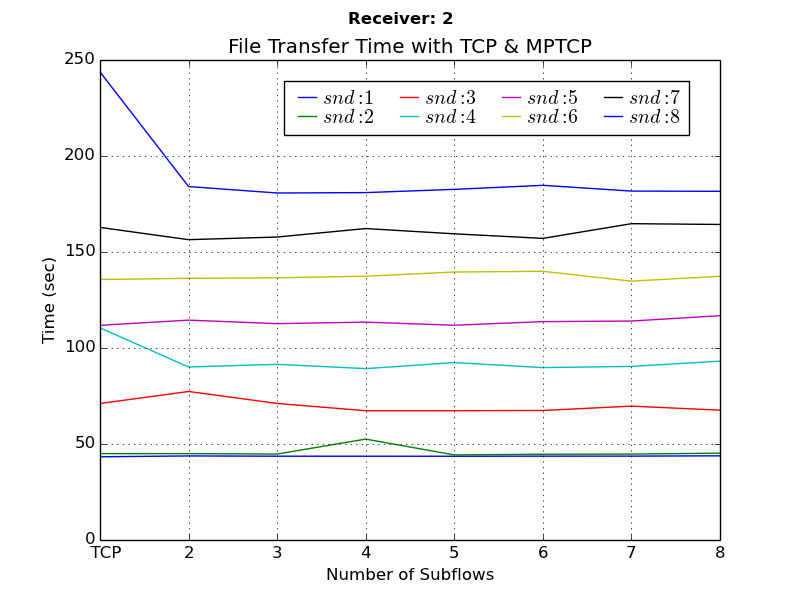
\includegraphics[width=\textwidth,height=3.8in]{images/rcv_2.png}
    \caption{2 receivers multiple senders.}
    \label{fig:rcv2}
  \end{figure}

  \begin{figure}
    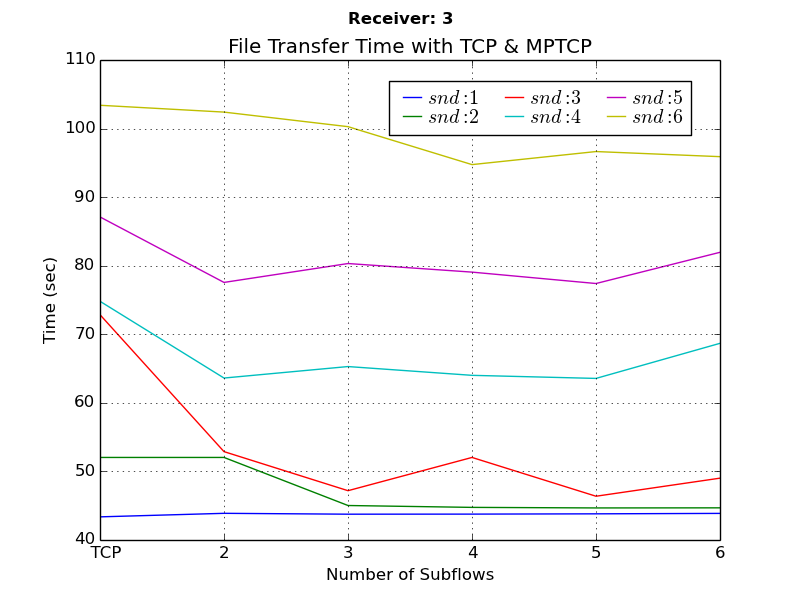
\includegraphics[width=\textwidth,height=3.8in]{images/rcv_3.png}
    \caption{3 receivers multiple senders.}
    \label{fig:rcv3}
  \end{figure}

  \begin{figure}
    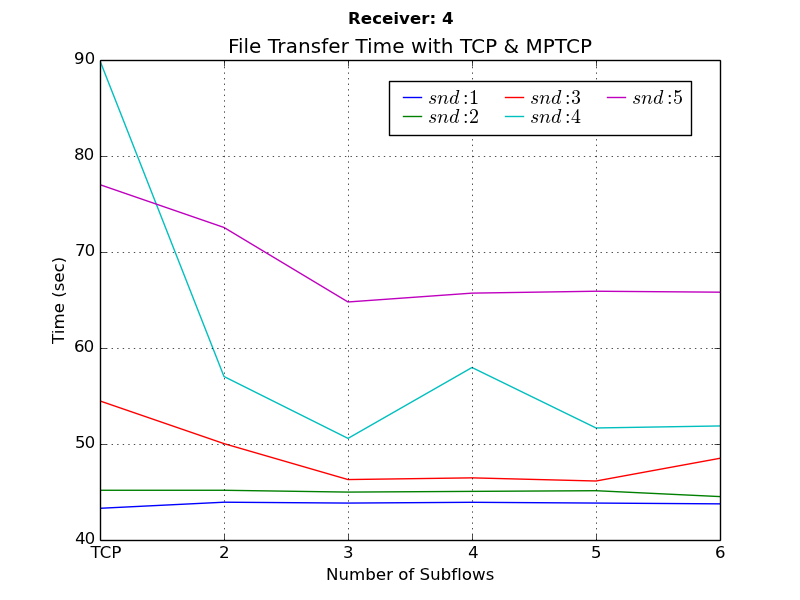
\includegraphics[width=\textwidth,height=3.8in]{images/rcv_4.png}
    \caption{4 receivers multiple senders.}
    \label{fig:rcv4}
  \end{figure}

  \begin{figure}
    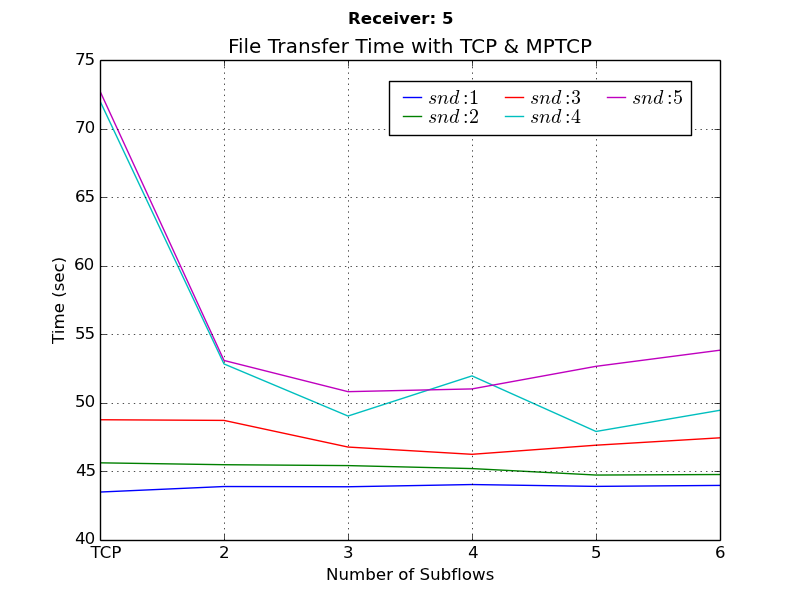
\includegraphics[width=\textwidth,height=3.8in]{images/rcv_5.png}
    \caption{5 receivers multiple senders.}
    \label{fig:rcv5}
  \end{figure}

  \begin{figure}
    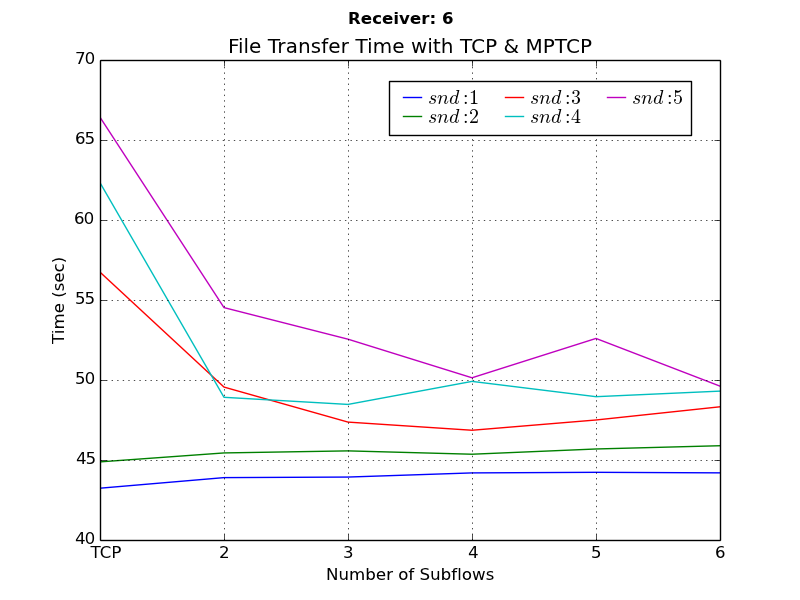
\includegraphics[width=\textwidth,height=3.8in]{images/rcv_6.png}
    \caption{6 receivers multiple senders.}
    \label{fig:rcv6}
  \end{figure}

  \begin{figure}
    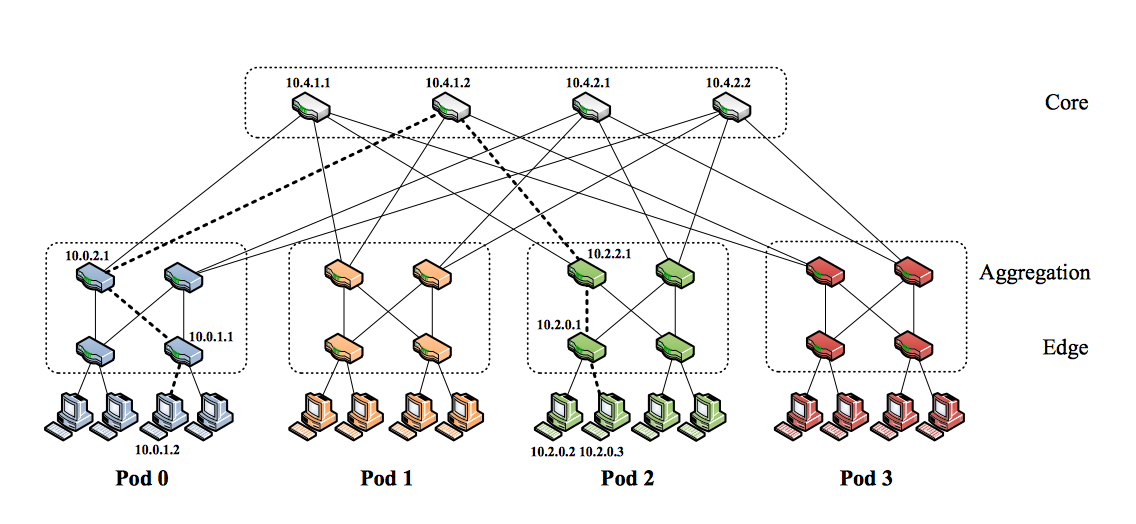
\includegraphics[width=\textwidth]{images/fattree.png}
    \caption{Fat Tree Topology with k=4.}
    \label{fig:ft}
  \end{figure}

  \begin{figure}
    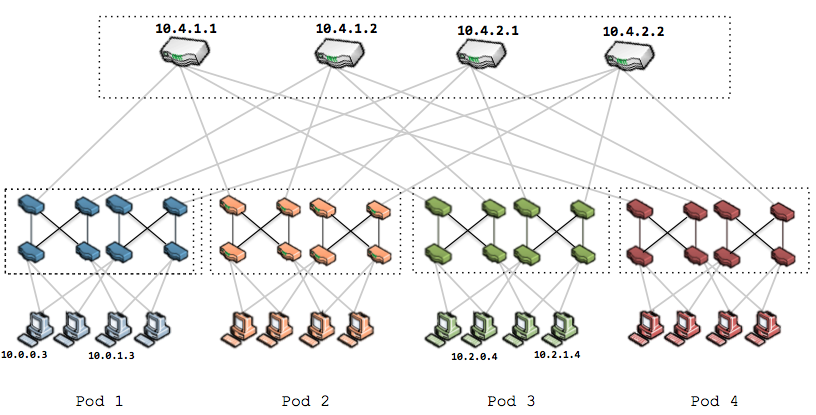
\includegraphics[width=\textwidth]{images/dht.png}
    \caption{Dual Homed Tree Topology with k=4.}
    \label{fig:dht}
  \end{figure}

\end{appendices}

\bibliography{report}{}
\bibliographystyle{plain}
\end{document}
